\documentclass[12pt]{article}
 \usepackage[margin=1in]{geometry} 
 \usepackage{graphicx}
\usepackage{amsmath,amsthm,amssymb,amsfonts}
 
\newcommand{\N}{\mathbb{N}}
\newcommand{\Z}{\mathbb{Z}}
 
\newenvironment{problem}[2][Problem]{\begin{trivlist}
\item[\hskip \labelsep {\bfseries #1}\hskip \labelsep {\bfseries #2.}]}{\end{trivlist}}
%If you want to title your bold things something different just make another thing exactly like this but replace "problem" with the name of the thing you want, like theorem or lemma or whatever
 
\begin{document}
 
%\renewcommand{\qedsymbol}{\filledbox}
%Good resources for looking up how to do stuff:
%Binary operators: http://www.access2science.com/latex/Binary.html
%General help: http://en.wikibooks.org/wiki/LaTeX/Mathematics
%Or just google stuff
 
\title{Production of long lived particles with charged leptons}
\author{Hao-Lin Li, Jiang-Hao Yu, Michael Ramsey-Musolf}
\maketitle
\section{Description of the Simplified Model}
In this simplified model we introduce three heavy neutrinos $N_1, N_2, N_3$ ($N_1$ lightest) and a right handed charged gauge boson $W_R$. The Lagrangian contain following new interactions:
\begin{eqnarray}
{\Delta\cal L}&=&\frac{g}{\sqrt{2}}W_L^\mu \left(\frac{M^2_{W_L}}{M^2_{W_R}}(\sin{2\beta})k_q\ \bar{u}_{iR} V^{CKMR}_{ij}\gamma^\mu d_{jR}+\frac{M^2_{W_L}}{M^2_{W_R}}(\sin{2\beta})k_l\ \bar{N}_{iR} (Y_{lN})_{ij}\gamma^\mu l_{jR} \right. \nonumber \\
&&\left. +\sqrt{\epsilon-\frac{M_{\nu}}{M_{N_1}}}k_l\ \bar{N}^c_{iR} (Y_{lN})_{ij}\gamma^\mu l_{jL}\right)\nonumber \\
&&+\frac{g}{\sqrt{2}}W_R^\mu \left(k_{Rq}\ \bar{u}_{iR} V^{CKMR}_{ij}\gamma^\mu d_{jR}+k_{Rl}\ \bar{N}_{iR} (Y_{lN})_{ij}\gamma^\mu l_{jR}\right)
\end{eqnarray}
where $g$ is the weak coupling constant, the ratio $M^2_{W_L}/M^2_{W_R}$ represents the scale of the mixing between $W_L$ and $W_R$, $\tan\beta=v_2/v_1$ is the ratio of the vacuum expectation value (vev) of two neutral scalar in the bi-doublet. $\epsilon=v_L/v_R$ is the ratio of the vev of left handed triplet and right handed triplet, the ratio $M_\nu/M_{N1}$ represents scale of the mixing between the left and right handed neutrino. The dimensionless parameters $k_q$, $k_l$, $k_{Rq}$, $k_{Rl}$ are set to 1 by default, the $3\time 3$ matrix $V^{CKMR}$ and $Y_{lN}$ are set to be identity by default, $M_{\nu}$ represents the scale of the mass of light neutrinos and set to be 0.1 eV by default.

\section{Production and Decay Processes}
We provide the following production and decay processes with corresponding \texttt{proc\_card} and \texttt{madspin\_card}:
\begin{center}
\begin{tabular}{c |c c}
    \hline
    \hline
    production of $N_1$& $p p \to \ell^{\pm} N_1$& \texttt{proc\_card\_N1l.dat}\\
    \hline
    decay of $N_1$& $N_1\to \ell^{\pm} j j$& \texttt{madspin\_card\_ljj.dat}\\
    & $N_1\to \ell^{\pm}\ell^{\mp}\nu$ & \texttt{madspin\_card\_3l\_MET.dat}\\
    \hline
    \hline
     production of $N_1$& $p p \to e^{+} N_1$& \texttt{proc\_card\_Nep.dat}\\
    \hline
    & $N_1\to e^+ \mu^- \nu $& \texttt{madspin\_card\_epmu.dat}\\
    decay of $N_1$& $N_1\to e^+ e^- \nu$ & \texttt{madspin\_card\_epe.dat}\\
    & $N_1\to e^- \mu^+ \nu$ & \texttt{madspin\_card\_emup.dat}\\
    \hline
    \hline
\end{tabular}
\end{center}


\section{Description of the Parameters}
\begin{center}
\begin{tabular}{c |c| c}
    \hline
    Parameter& Default Value& Description \\
    \hline
    \texttt{mN1}, \texttt{mN2}, \texttt{mN3}& $40,10^{12},10^{14} {\rm GeV}$ & The mass of heavy neutrinos, only the lightest one is active \\
    \hline
    \texttt{MWR}, \texttt{WWR} & 15000, 100 {\rm GeV} & The mass and width of the right handed $W$ boson \\
    \hline
    \texttt{kq}, \texttt{kl}& 1.0, 1.0& scaling factor of the $W_L$ couplings for quark and lepton\\
    \hline 
    \texttt{kRq}, \texttt{kRl}& 1.0, 1.0& scaling factor of the $W_R$ couplings for quark and lepton\\
    \hline
    \texttt{Mnu} & 0.1 {\rm eV}& The mass scale of light neutrino\\
    \hline
     \texttt{tanb} & 0.1 & ratio of $v_2$ and $v_1$\\
    \hline
     \texttt{epsi} & 0.0 & ratio of $v_L$ and $v_R$\\
    \hline
    \texttt{VCKMR} &Idendity& Right handed quark CKM matrix\\
    \hline
    \texttt{YlN} &Idendity& Right handed lepton mixing matrix\\
    \hline
\end{tabular}
\end{center}

\vspace{5mm}

We also provide a plot to illustrate the length of the displaced vertex produced by the lightest heavy neutrino $N_1$ in the $M_{W_R}$ vs $M_{N_1}$ plane, all the other parameters are set to their default values.
\begin{figure}[h!]
 \centering
 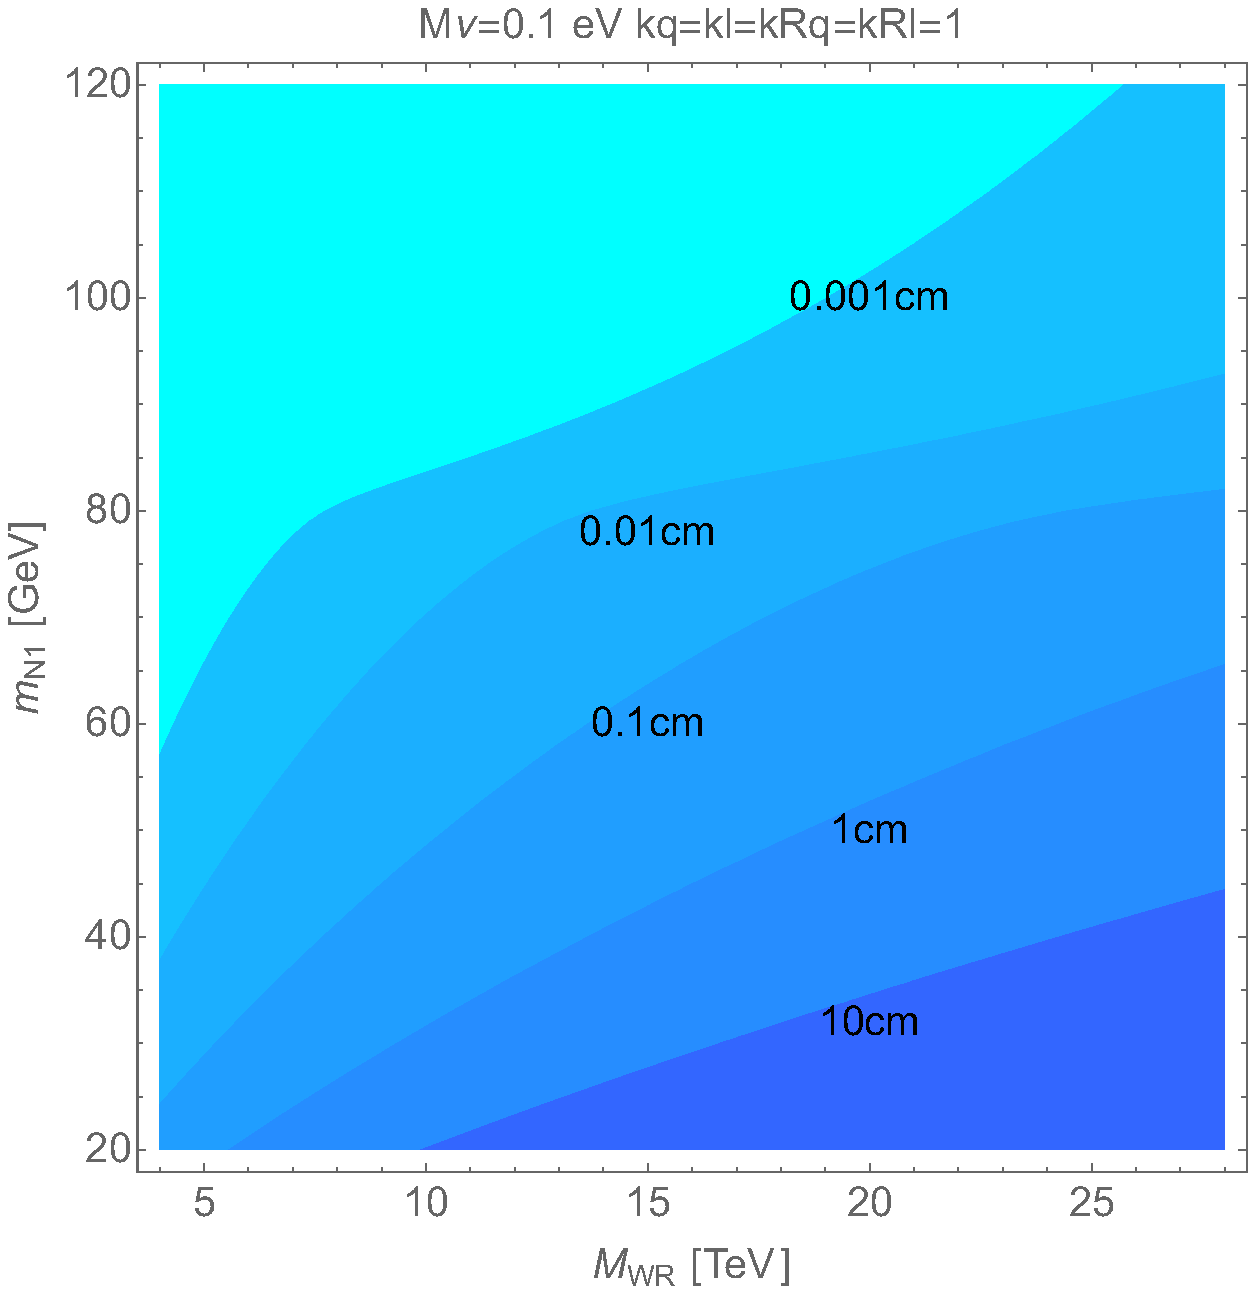
\includegraphics[width=0.5\textwidth]{decaylength.pdf}
 \caption{The contour of the length of the displaced vertex.}
 \end{figure}

\section{User Guide}
One should first copy the model file \texttt{ChargeWN\_UFO} to the \texttt{models} folder in the Madgraph. Then one can use \texttt{./bin/mg5\_aMC proc\_card\_N1l.dat} to produce the process folder \texttt{LLP\_N1l}. Go into the process folder \texttt{LLP\_N1l} and copy the madspin card into the \texttt{Cards} folder and rename as \texttt{madspin\_card.dat} for different process. One can use the \texttt{proc\_card\_Nep.dat} in the similar way to specify the flavor of the leptons in the decay chains. 

For the simplest use, one only need to change the mass of right handed $W_R$ boson, \texttt{MWR} and the mass of the lightest heavy neutrino $N_1$, ``\texttt{mN1}" to obtain different travel length of the long-lived particle. Every time the user changes the parameters in the \texttt{param\_card.dat}, one should set the width ``\texttt{WN1}" of the longlived particle to \texttt{Auto} such that Madgraph will calculate the Width of $N_1$ automatically.

We also provide a python script ``mgrun" to help to do the parameter scan. people needs to first generate a table of parameters by themselves in the following format:
\begin{center}
\begin{tabular}{c c c c}

    mN1 & WN1 & MWR & ...\\
    100 & Auto & 6000 & ... \\
	200 & Auto & 6000 & ... \\
    ... & ... & ... & ...
\end{tabular}
\end{center}
where the first line are the names of the parameters you want to scan, and the following lines are the value of the parameters. To scan this table one only need to copy the script ``mgrun" and the ``table" to the process folder like \texttt{LLP\_N1l} you generated, and run the following line in the terminal:
\begin{center}
mgrun\ \  ./\ \  ./table.txt
\end{center}
The first argument is the path of your process folder, if one use this script on a cluster one can replace ``./'' to the global path of your process folder.


\end{document}